\documentclass[a4paper, 14pt]{extarticle}

\usepackage{setspace}
\usepackage{titlesec}

% add cyrillic
\usepackage[utf8]{inputenc}
\usepackage[russian, ukrainian]{babel}

% line spacing
\onehalfspacing

% margins
\usepackage[top=25mm, right=25mm, bottom=15mm, left=25mm]{geometry}

% this is a global declaration that changes the appearance of the section command
\titleformat{\section}{\large\scshape\raggedright}{}{0em}{}

% paragraph indents
\usepackage{parskip}
\setlength{\parindent}{15pt}
% indent first paragraph
\usepackage{indentfirst}

% packages for images
\usepackage{graphicx}
\usepackage{float}

\begin{document}

\begin{titlepage}
  \vspace*{\fill}

  \begin{center}
    {\Large Звіт по проходженню наукової практики}\\[.5cm]
    {\Large 
      Іван Сергієнко\\
      група ФФ-11\\[.4cm]
      ФТІ, КПІ}\\[.4cm]
    \date{}
  \end{center}
  \vspace*{\fill}
\end{titlepage}


\section{Вступ}
Під час практики в інституті фізики напіпровідників ім. В.Є. Лашкарьова НАН України я ознайомився з методами нанесення тонких плівок та відповідним обладнанням. За моєї участі бли отримані тонкі плівки алюмінію на скляних підклаках дзеркала. Також я ознайомився з методами вимірювання люмінісценсції та відповідним обладнанням. Були проведені вимірювання електролюмінісцентих легованих плівок ZnS. Також я ознайомився з методом атомно-силової мікроскопії, за допомогою якої була досліджена морфологія поверхні плівок алюмінію на склі. Я опрацював відповідну літературу по цим напрямках. В рамках практики я розробляв програму розрахунку оптичних сталих по спектрам пропускання та відбивання (за методом Сванполя).
\newpage
\section{1. Нанесення тонких плівок}

В процесі ознайомчої практики я брав участь в роботах по нанесеннюю на різноманітні підкладки тонких плівок металів та неметалів шляхом резистивного випаровування у вакуумі.

Роботи проводились на установках УВН2М-1 і ВУ-1А. Попередньо я ознайомився з будовою вказаних вакуумних установок: конструкцією відкачної системи з насосами попереднього та остаточного вакуума, камери напилення і електричної частини.

На установці УВН2М-1 були нанесені плівки $Al$ товщиною 1300-1700 $\mbox{\normalfont\AA}$ на підкладці скла АК-7. При нанесенні  $Al$ був виготовлений випаровувач з $W$-дроту діаметром 1мм з безпосереднім підігрівом. Струм пропускався через $W$-випаровувач, на якому знаходився $Al$-матеріал. При нагріванні до температури $\sim 600 ^{\circ}C$ $Al$ розплавляється, легко розтікається по поверхні випаровувача і при температурі $\sim 1000 ^{\circ}C$ починає випаровуватися. Процес відбувається у вакуумній камері, відкачанній до тиску порядку $10^{-5}$ мм рт. ст.

Нанесені на підкладку плівки $Al$ світлосірого кольору. Міцність зчеплення алюмінієвих плівок зі склом (попередньо очищеним) дуже велика. Ці плівки є доволі тверді і корозійно стійки через постійну присутність самовільно виникаючої в повітрі поверхневої плівки окису алюмінію ($\sim 80 {\mbox{\normalfont\AA}}$).

При нанесенні плівок $SiO$ на установці ВУ-1А методом резистивного випаровування я був ознайомлений з влаштуванням контролю оптичних товщин тонких плівок в процесі їх нанесення.

Принцип дії пристрою оснований на фотоелектричному методі реєстрації променистого потоку відбитого від зразку, який напиляється. При цьому про оптичну товщину матеріалу, що напиляється, можно судити по зміні відбиття від зразку. Екстремальним значенням відбиття відповідає товщини плівки $(d)$, кратна значенням $n \cdot \frac{\lambda}{4}$, де $\lambda$ - довжина хвилі випромінення на виході монохроматора, $n$ - коефіцієнт заломлення речовини, що наноситься.

З використанням цього пристрою були нанесені плівки $SiO$ товщиною $1800-2000 \mbox{\normalfont\AA}$.

\newpage

\section{2. Атомно-силова мікроскопія}
\begin{center}
  \begin{figure}[H]
    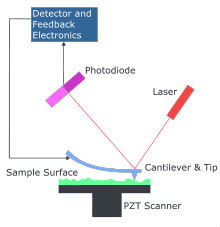
\includegraphics[scale=.8]{./img/afm.jpg}
  \end{figure}
\end{center}

Принцип дії атомно-силового мікроскопу базується на силах, що виникають між атомами на близьких відстанях. Це сила відштовхування Паулі, викликана перекриттям електронних орбіталей, та сила притягування Ван Дер Ваальса. Разом вони формують потенціал Леннарда-Джонса. Скануючий щуп мікроскопа вносять в зону дії описаних сил, від чого він деформується. Деформація фіксується датчиками і програмне забезпечення відновлює зображення поверхні по відомим значенням діючої на щуп сили.

Високоточне переміщення поверхні під щупом забезпечують п'єзоелектричні елементи, які змінюють свою довжину в залежності від прикладеної напруги. Рухаючись над нерівною поверхнею, щуп підіймається і опускається, і ці дуже малі вертикальні переміщення детектуються за допомогою лазерного променя, який падає на верхню поверхню консольної балки з прикріпленим дзеркалом. Хоча вертикальні переміщення дзеркала дуже малі, відбитий від нього промінь відхиляється на кут, досить значний, щоб його можна було виміряти за допомогою матричного фотодетектора. Отриманий сигнал аналізується за допомогою електроніки й перетворюється в зображення поверхні. Для забезпечення постійної сили між поверхнею та щупом і запобігання пошкоджень, використовується електронний механізм зворотного зв'язку.

\newpage

За допомогою атомно-силового мікроскопу було отримане зображення нанесеної шляхом випаровування плівки $Al$:
\begin{figure}[H]
  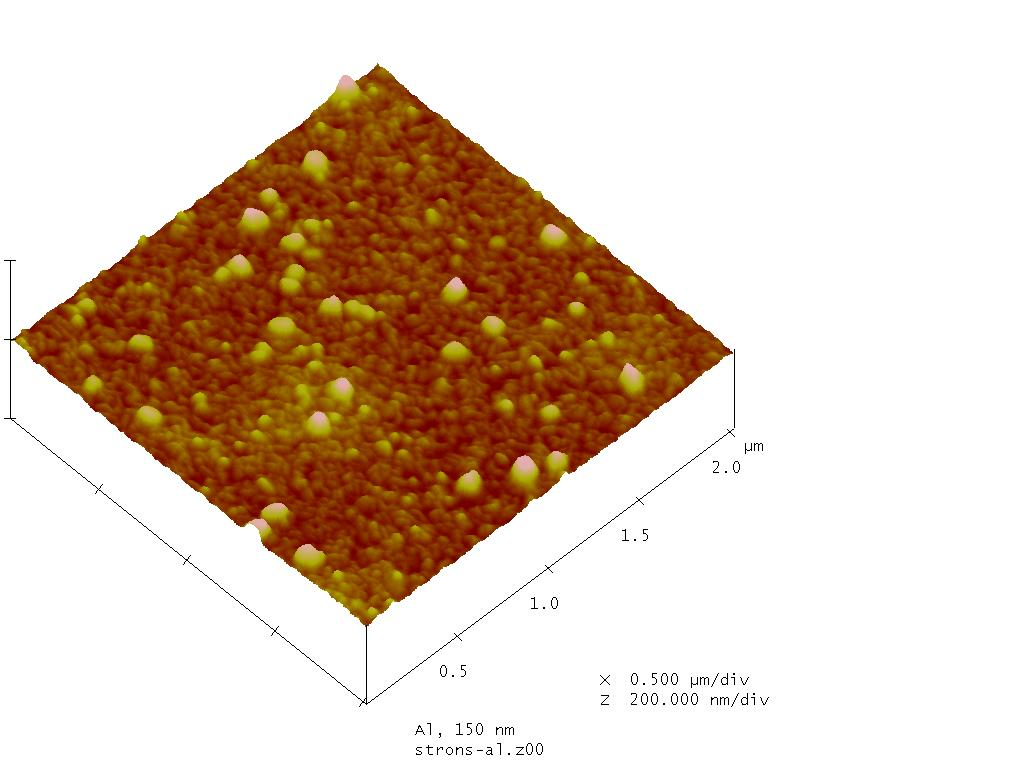
\includegraphics[width=130mm]{./img/afm_al/afm-al-6.jpg}
\end{figure}

\begin{figure}[H]
  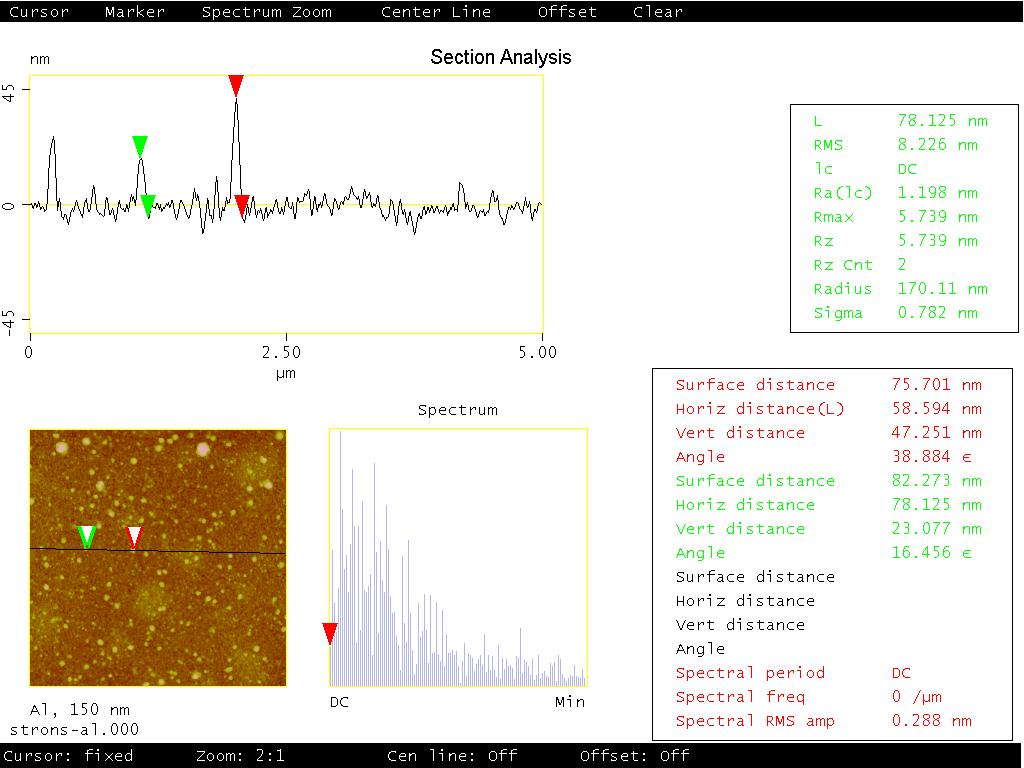
\includegraphics[width=130mm]{./img/afm_al/afm-al-4.jpg}
\end{figure}

\newpage

\section{3. Тонкоплівкові електролюмінісцентні структури}
Тонкоплівкові електролюмінісцентні структури представляють собою послідовно нанесені на скляні підкладки шари:

\begin{figure}[H]
  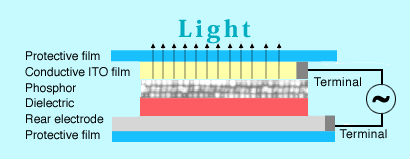
\includegraphics[width=120mm]{./img/electroluminiscentTape.jpg}
\end{figure}

\begin{enumerate}
  \item прозорий електрод $ITO$ $(In_2 O_3: Sn)$ нижній електрод, через який і спостерігається світіння;
  \item нижній діелектричний шар $SiO_2/Al_2O_3$ (270 нм);
  \item елетролюмінісцентний шар $ZnS:Mn$ (600-650 нм);
  \item верхній діелектричний шар $Al_2 O_3/SiO$;
  \item верхній електрод-плівка $Al$.
\end{enumerate}

Електролюмінісценція (ЕЛ) - це люмінісценція, що збуджується електричним полем, здатним змінити потенціальну або кінетичну енергію електронів та дірок. По механізму збудження вона підрозділяється на інжекційну і передпробійну. Передпробійна ЕЛ виникає в сильних електричних полях ($\geq 10^5$ В/см). Найбільше розповсюджена та має найбільше практичне значення ударна ЕЛ, особливо в тонкоплівкових МПДМ та МДПДМ структурах. В них робочий шар - це високоомний ($10^5 - 10^{12}$ ом $\cdot$ см) напівпровідник або напівізолятор, що містить центри світіння, наприклад, ZnS:Mn, ZnS:РЗЕ (Su, Tb, та ін.), укладений між двома діелектриками. В перепробійній ЕЛ існують наступні основні стадії:
\begin{enumerate}
  \item Інжекція вільний носіїв в область сильного поля з електродів та/або поверхневих станів на границі діелектрик-ZnS, або генерація їх в результаті удраної або тунельної іонізації глибоких донорів, пасток і т.д.
  \item прискорення носіїв до необхідної енергії.
  \item Збудження центрів світіння безпосередньо при непружному зіткненні.
  \item Випромінення.
\end{enumerate}
Найбільш ефективними є внутрішньоцентрові випромінюючі переходи в перехідних $(Mn^{2+})$ або РЗ йонах ($Tb^{3+}, Su^{3+}$, та ін.).

\newpage

\section{Висновок}
Дякуючи практиці я познайомився з процесом роботи наукової установи, високотехнологічним обладнанням, сучасними методами розрахунку параметрів тонких оптичних плівок. Завдяки цьому у мене склалося уявлення про роботу науковців та призначення випускників моєї спеціальності. Я отримав перший досвід вивчення наукових статей та літератури. Збільшилося моє розуміння слова "високотехнологчіний".

\end{document}
